\documentclass[]{article}

\usepackage[margin=0.5in]{geometry}
%\usepackage[paperwidth=5.5in, paperheight=8.5in]{geometry}
\usepackage{graphicx}
\usepackage{float}
\usepackage{amsmath}
\usepackage{amssymb}
\usepackage{hyperref}
\usepackage{multirow}

\pagestyle{plain}

\begin{document}

%% Rabbit 10 = Subject 1
%% Rabbit 9 = Subject 2

\section{Methods}
This section describes the computational analysis performed on the data.
For all analog channels, the data was first processed with a high-pass Butterworth filter with a stopband-edge frequency of 2 Hz, a passband-edge frequency of 10 Hz, a stopband attenuation of 90 dB, and passband ripple of 1 dB.
Afterwards, cardiac removal is performed on all channels using the methods described in section \ref{section:cardiac}.

\subsection{Visual Evoked Potential}
During the VEP experiments, the digital in channel was synchronized with the LED turning on and off.
For both the on and off edges, the signal from the electrodes were aligned to compute the mean signal and confidence intervals.
[Some edges were removed if the the timing was inconsistent for some reason.]
The displayed confidence intervals are a 95\% bootstrapped value for the mean.
All VEP trials include between 153 and 208 events.

\subsection{Steady-State Visual Evoked Potential}
During the SSVEP experiment, and LED was flashed at 40 Hz with a 50\% duty cycle.
For both a resting state and experimental period, Welsh's method was used to compute the power spectral density with a window length of 2 seconds and an overlap of 25\%.
The ratio of the experimental power with the resting state power at each frequency is shown.
All data within 3 Hz of a 60 Hz harmonics are excluded due to showing heavy artifacts from electrical equipment.
The background data includes data more than 3 Hz away from harmonics of 40 Hz, and the harmonic data takes the maximum power at a frequency within 3 Hz of each harmonic.
All experimental measurements lasted between 22.5 seconds and 57.0 seconds, and all resting state measurements lasted between 28.8 seconds and 60.7 seconds.
\subsection{Steady-State Auditory Evoked Potential}
[Same processing as SSVEP]
All experimental measurements lasted between 29.0 seconds and 59.2 seconds, and all resting state measurements lasted between 4.4 seconds and 59.0 seconds.
[Subject 2 has very short resting state measurements for SSAEP - shortest for subject 1 is 28.4 seconds]
\subsection{Cardiac Artifacts and Removal}
The cardiac data is high-passed.
The maximum in a 0.18 second interval is considered the R peak.
The segments are split 0.63 between the R peaks (this is so that the P-wave and T-wave end up on opposite sides).
The mean is computed for each time step relative to the R peak, and a zero is averaged in for trials that do not extend that far out (the R peaks are not exactly equally centered).
In some sense, this indicates uncertainty in what the cardiac artifacts are at that time, so a smaller adjustment is made.
The mean for the cardiac shape is then subtraced out from each electrode.
\label{section:cardiac}
\begin{figure}[H]
\begin{center}
\includegraphics[scale=1.0]{surgical_methods.pdf}
\caption{Surgical approach, anatomy imaging.}
\label{fig:surgical}
% Figure 1
\end{center}
\end{figure}

\setlength{\tabcolsep}{2pt}
\begin{figure}[H]
\begin{center}
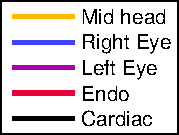
\includegraphics[]{../config/legend2.pdf} % TODO: vertical center
\hspace{0.3cm}
\begin{tabular}{c|cc|cc}
& \multicolumn{2}{c|}{Experiment} & \multicolumn{2}{c}{Control} \\
& Subject 1 & Subject 2 & Subject 1 & Subject 2 \\
\hline
\raisebox{-0.5\height}{\rotatebox{90}{VEP On}} &
\raisebox{-0.5\height}{\includegraphics[scale=0.32]{../vep/matlab_data/_Thu_15_05_2014_11_57_42_vep__labelled-crop.pdf}} &
\raisebox{-0.5\height}{\includegraphics[scale=0.32]{../vep/matlab_data/_Tue_06_05_2014_11_17_10_vep_-crop.pdf}} &
\raisebox{-0.5\height}{\includegraphics[scale=0.32]{../vep/matlab_data/_Thu_15_05_2014_12_15_47_vep_ctr-crop.pdf}} &
\raisebox{-0.5\height}{\includegraphics[scale=0.32]{../vep/matlab_data/_Tue_06_05_2014_11_25_22_vep_-crop.pdf}} \\
\raisebox{-0.5\height}{\rotatebox{90}{VEP Off}} &
\raisebox{-0.5\height}{\includegraphics[scale=0.32]{../vep/matlab_data/_Thu_15_05_2014_11_57_42_vep__off_labelled-crop.pdf}} &
\raisebox{-0.5\height}{\includegraphics[scale=0.32]{../vep/matlab_data/_Tue_06_05_2014_11_17_10_vep__off-crop.pdf}} &
\raisebox{-0.5\height}{\includegraphics[scale=0.32]{../vep/matlab_data/_Thu_15_05_2014_12_15_47_vep_ctr_off-crop.pdf}} &
\raisebox{-0.5\height}{\includegraphics[scale=0.32]{../vep/matlab_data/_Tue_06_05_2014_11_25_22_vep__off-crop.pdf}} \\
\raisebox{-0.5\height}{\rotatebox{90}{SSAEP 86 Hz}} &
\raisebox{-0.5\height}{\includegraphics[scale=0.32]{../ssavep/matlab_data/_Thu_15_05_2014_14_26_54_ssaep_86_labelled-crop.pdf}} &
\raisebox{-0.5\height}{\includegraphics[scale=0.32]{../ssavep/matlab_data/_Tue_06_05_2014_11_37_22_ssaep_86-crop.pdf}} &
\raisebox{-0.5\height}{\includegraphics[scale=0.32]{../ssavep/matlab_data/_Thu_15_05_2014_12_26_26_ssaep_ctr_86-crop.pdf}} &
\raisebox{-0.5\height}{\includegraphics[scale=0.32]{../ssavep/matlab_data/_Tue_06_05_2014_11_42_15_ssaep_86-crop.pdf}} \\
\raisebox{-0.5\height}{\rotatebox{90}{SSVEP 40 Hz}} &
\raisebox{-0.5\height}{\includegraphics[scale=0.32]{../ssavep/matlab_data/_Thu_15_05_2014_14_20_24_ssvep_40_labelled-crop.pdf}} &
\raisebox{-0.5\height}{\includegraphics[scale=0.32]{../ssavep/matlab_data/_Tue_06_05_2014_11_14_51_ssvep_40-crop.pdf}} &
\raisebox{-0.5\height}{\includegraphics[scale=0.32]{../ssavep/matlab_data/_Thu_15_05_2014_12_13_26_ssvep_ctr_40-crop.pdf}} &
\raisebox{-0.5\height}{\includegraphics[scale=0.32]{../ssavep/matlab_data/_Tue_06_05_2014_11_23_01_ssvep_40-crop.pdf}}
\end{tabular}
\caption{Performance of the electrodes at the optimal location for the endovascular location compared with the performance on the live control trials. The SSAEP and SSVEP experimental trials for Subject 1 are shown for the mid-basilar location. All other performances are shown at the basilar tip position. In each of the experiments, all experimental trials elicited a much larger response than the control experiments, which indicates that true non-artifactual responses were recorded. In addition, the endovascular electrode achieved superior signals compared to the scalp electrodes for the VEP and SSAEP experiments.}
\label{fig:both}
% Figure 2
\end{center}
\end{figure}
\setlength{\tabcolsep}{6pt}

\setlength{\tabcolsep}{2pt}
\begin{figure}[H]
\begin{center}
\begin{tabular}{c|cccc|cc}
         & \multicolumn{4}{c|}{Experiment}                       & \multicolumn{2}{c}{Control} \\
         &             &             &             &             & Live         & Dead \\
\hline
Location & Basilar Tip & Mid-Basilar & VB Junction & Basilar Tip & Basilar Tip  & Basilar Tip \\
Time     & 11:57:42    & 14:13:26    & 15:54:54    & 16:47:47    & 12:15:47     & 17:22:22 \\
Time     & 0:00:00 & 2:15:44 & 3:57:12 & 4:50:05 & 0:18:05 & 5:24:40 \\ % TODO: time relative to anesthesia? relative to surgery
\hline
\raisebox{-0.5\height}{\rotatebox{90}{VEP On}} &
\raisebox{-0.5\height}{\includegraphics[scale=0.32]{../vep/matlab_data/_Thu_15_05_2014_11_57_42_vep__labelled-crop.pdf}} &
\raisebox{-0.5\height}{\includegraphics[scale=0.32]{../vep/matlab_data/_Thu_15_05_2014_14_13_26_vep_-crop.pdf}} &
\raisebox{-0.5\height}{\includegraphics[scale=0.32]{../vep/matlab_data/_Thu_15_05_2014_15_54_54_vep_-crop.pdf}} &
\raisebox{-0.5\height}{\includegraphics[scale=0.32]{../vep/matlab_data/_Thu_15_05_2014_16_47_47_vep_-crop.pdf}} &
\raisebox{-0.5\height}{\includegraphics[scale=0.32]{../vep/matlab_data/_Thu_15_05_2014_12_15_47_vep_ctr-crop.pdf}} &
\raisebox{-0.5\height}{\includegraphics[scale=0.32]{../vep/matlab_data/_Thu_15_05_2014_17_22_22_vep_-crop.pdf}} \\
\raisebox{-0.5\height}{\rotatebox{90}{VEP Off}} &
\raisebox{-0.5\height}{\includegraphics[scale=0.32]{../vep/matlab_data/_Thu_15_05_2014_11_57_42_vep__off_labelled-crop.pdf}} &
\raisebox{-0.5\height}{\includegraphics[scale=0.32]{../vep/matlab_data/_Thu_15_05_2014_14_13_26_vep__off-crop.pdf}} &
\raisebox{-0.5\height}{\includegraphics[scale=0.32]{../vep/matlab_data/_Thu_15_05_2014_15_54_54_vep__off-crop.pdf}} &
\raisebox{-0.5\height}{\includegraphics[scale=0.32]{../vep/matlab_data/_Thu_15_05_2014_16_47_47_vep__off-crop.pdf}} &
\raisebox{-0.5\height}{\includegraphics[scale=0.32]{../vep/matlab_data/_Thu_15_05_2014_12_15_47_vep_ctr_off-crop.pdf}} &
\raisebox{-0.5\height}{\includegraphics[scale=0.32]{../vep/matlab_data/_Thu_15_05_2014_17_22_22_vep__off-crop.pdf}} \\
\raisebox{-0.5\height}{\rotatebox{90}{SSAEP 86 Hz}} &
\raisebox{-0.5\height}{\includegraphics[scale=0.32]{../ssavep/matlab_data/_Thu_15_05_2014_12_31_02_ssaep_86_labelled-crop.pdf}} &
\raisebox{-0.5\height}{\includegraphics[scale=0.32]{../ssavep/matlab_data/_Thu_15_05_2014_14_26_54_ssaep_86-crop.pdf}} &
\raisebox{-0.5\height}{\includegraphics[scale=0.32]{../ssavep/matlab_data/_Thu_15_05_2014_16_12_19_ssaep_86-crop.pdf}} &
\raisebox{-0.5\height}{\includegraphics[scale=0.32]{../ssavep/matlab_data/_Thu_15_05_2014_16_58_34_ssaep_86-crop.pdf}} &
\raisebox{-0.5\height}{\includegraphics[scale=0.32]{../ssavep/matlab_data/_Thu_15_05_2014_12_26_26_ssaep_ctr_86-crop.pdf}} &
\raisebox{-0.5\height}{\includegraphics[scale=0.32]{../ssavep/matlab_data/_Thu_15_05_2014_17_12_38_ssaep_86-crop.pdf}} \\
\raisebox{-0.5\height}{\rotatebox{90}{SSVEP 40 Hz}} &
\raisebox{-0.5\height}{\includegraphics[scale=0.32]{../ssavep/matlab_data/_Thu_15_05_2014_12_08_22_ssvep_40_labelled-crop.pdf}} &
\raisebox{-0.5\height}{\includegraphics[scale=0.32]{../ssavep/matlab_data/_Thu_15_05_2014_14_20_24_ssvep_40-crop.pdf}} &
\raisebox{-0.5\height}{\includegraphics[scale=0.32]{../ssavep/matlab_data/_Thu_15_05_2014_16_02_44_ssvep_40-crop.pdf}} &
\raisebox{-0.5\height}{\includegraphics[scale=0.32]{../ssavep/matlab_data/_Thu_15_05_2014_16_38_47_ssvep_40-crop.pdf}} &
\raisebox{-0.5\height}{\includegraphics[scale=0.32]{../ssavep/matlab_data/_Thu_15_05_2014_12_13_26_ssvep_ctr_40-crop.pdf}} &
\raisebox{-0.5\height}{\includegraphics[scale=0.32]{../ssavep/matlab_data/_Thu_15_05_2014_17_18_01_ssvep_40-crop.pdf}}
\end{tabular}
\caption{Demonstration of position dependence for Subject 1. The performance of the endovascular electrode varies as its location is changed. The performance is consistent between the two basilar tip trials. The responses measured during the experimental trials are much larger than the signals during the control trials.}
\label{fig:position}
% Figure 3
\end{center}
\end{figure}
\setlength{\tabcolsep}{6pt}

\begin{figure}[H]
\begin{center}
\begin{tabular}{cc}
\includegraphics[scale=0.5]{impedance.pdf}
\end{tabular}
\caption{Impedance characterization.}
\label{fig:impedance}
% Figure 4
\end{center}
\end{figure}

%\begin{figure}[H]
%\begin{center}
%\begin{tabular}{cc}
%\multirow{2}{*}{
%\begin{tabular}{ccc}
%Raw Trace & VEP Aligned & \\
%\raisebox{-0.5\height}{\includegraphics[scale=0.32]{../qrs/matlab_data/_Thu_15_05_2014_14_13_26_vep__start-crop.pdf}} &
%\raisebox{-0.5\height}{\includegraphics[scale=0.32]{../vep/matlab_data/_Thu_15_05_2014_14_13_26_vep__cardiac_labelled-crop.pdf}} &
%\\
%\raisebox{-0.5\height}{\includegraphics[scale=0.32]{../qrs/matlab_data/_Thu_15_05_2014_14_13_26_vep__end-crop.pdf}} &
%\raisebox{-0.5\height}{\includegraphics[scale=0.32]{../vep/matlab_data/_Thu_15_05_2014_14_13_26_vep__labelled-crop.pdf}} &
%\end{tabular}} &
%\raisebox{-0.5\height}{cardiac aligned avg vep + EKG} \\
%& \raisebox{-0.5\height}{\includegraphics[scale=0.32]{../qrs/matlab_data/_Thu_15_05_2014_14_13_26_vep__qrs-crop.pdf}} \\
%%\raisebox{-0.5\height}{contaminated raw trace + cardiac} &
%%\raisebox{-0.5\height}{VEP aligned contaminated EKG} &
%%\raisebox{-0.5\height}{vep aligned cleaned} &
%%\raisebox{-0.5\height}{raw cleaned} &
%%\raisebox{-0.5\height}{\includegraphics[scale=0.32]{../qrs/matlab_data/_Thu_15_05_2014_14_13_26_vep__end-crop.pdf}}
%\end{tabular}

%\begin{figure}[H]
%\begin{center}
%\begin{tabular}{cccc}
%& Raw Trace & VEP Aligned & cardiac aligned avg vep + EKG \\
%\raisebox{-0.5\height}{\rotatebox{90}{Contaminated}} &
%\raisebox{-0.5\height}{\includegraphics[scale=0.32]{../qrs/matlab_data/_Thu_15_05_2014_14_13_26_vep__start-crop.pdf}} &
%\raisebox{-0.5\height}{\includegraphics[scale=0.32]{../vep/matlab_data/_Thu_15_05_2014_14_13_26_vep__cardiac_labelled-crop.pdf}} &
%\raisebox{-0.5\height}{\multirow{2}{*}{\includegraphics[scale=0.64]{../qrs/matlab_data/_Thu_15_05_2014_14_13_26_vep__qrs-crop.pdf}}} \\
%\raisebox{-0.5\height}{\rotatebox{90}{Cleaned}} &
%\raisebox{-0.5\height}{\includegraphics[scale=0.32]{../qrs/matlab_data/_Thu_15_05_2014_14_13_26_vep__end-crop.pdf}} &
%\raisebox{-0.5\height}{\includegraphics[scale=0.32]{../vep/matlab_data/_Thu_15_05_2014_14_13_26_vep__labelled-crop.pdf}} &
%\end{tabular}

\begin{figure}[H]
\begin{center}
\begin{tabular}{cc|cc}
\raisebox{-0.5\height}{\multirow{3}{*}{
\begin{tabular}{c}
Cardiac-Aligned  Measurements \vspace{0.7cm} \\
\includegraphics[scale=0.64]{../qrs/matlab_data/_Thu_15_05_2014_14_13_26_vep__qrs-crop.pdf}
\end{tabular}
}} &
& Raw Trace & VEP-Aligned \\
\hline
&
\raisebox{-0.5\height}{\rotatebox{90}{Contaminated}} &
\raisebox{-0.5\height}{\includegraphics[scale=0.32]{../qrs/matlab_data/_Thu_15_05_2014_14_13_26_vep__start-crop.pdf}} &
\raisebox{-0.5\height}{\includegraphics[scale=0.32]{../vep/matlab_data/_Thu_15_05_2014_14_13_26_vep__cardiac_labelled-crop.pdf}} \\
&
\raisebox{-0.5\height}{\rotatebox{90}{Cleaned}} &
\raisebox{-0.5\height}{\includegraphics[scale=0.32]{../qrs/matlab_data/_Thu_15_05_2014_14_13_26_vep__end-crop.pdf}} &
\raisebox{-0.5\height}{\includegraphics[scale=0.32]{../vep/matlab_data/_Thu_15_05_2014_14_13_26_vep__labelled-crop.pdf}} \\
\end{tabular}
\caption{Cardiac contamination and cleaning. The cardiac aligned measurements shows the mean and 95\% bootstrap confidence intervals for 1076 segments of data. The endovascular electrode is located at the mid-basilar location, which demonstrated the largest contamination from cardiac activity. The P-wave, QRS complex, and T-wave are all visible in the signal from the cardiac electrode. The raw trace show highly repeatable cardiac artifacts in the endovascular electrode, which are removed in the cleaned version. The VEP-aligned data has the same general trend before and after cardiac artifacts are accounted for, but the confidence intervals are much smaller after accounting for cardiac artifacts.}
\label{fig:cardiac}
% Figure 5
\end{center}
\end{figure}

\section*{Figure Information}
This section is information about which trials where used for the figures and some information about the trials.
\begin{table}[H]
\begin{center}
\begin{tabular}{c|cc|cc}
& \multicolumn{2}{c|}{Experiment} & \multicolumn{2}{c}{Control} \\
& Subject 1 & Subject 2 & Subject 1 & Subject 2 \\
\hline
\raisebox{-0.5\height}{\rotatebox{90}{VEP On}} &
../vep/matlab\_data/\_Thu\_15\_05\_2014\_11\_57\_42\_vep\_\_labelled-crop.pdf &
../vep/matlab\_data/\_Tue\_06\_05\_2014\_11\_17\_10\_vep\_-crop.pdf &
../vep/matlab\_data/\_Thu\_15\_05\_2014\_12\_15\_47\_vep\_ctr-crop.pdf &
../vep/matlab\_data/\_Tue\_06\_05\_2014\_11\_25\_22\_vep\_-crop.pdf \\
\raisebox{-0.5\height}{\rotatebox{90}{VEP Off}} &
../vep/matlab\_data/\_Thu\_15\_05\_2014\_11\_57\_42\_vep\_\_off\_labelled-crop.pdf &
../vep/matlab\_data/\_Tue\_06\_05\_2014\_11\_17\_10\_vep\_\_off-crop.pdf &
../vep/matlab\_data/\_Thu\_15\_05\_2014\_12\_15\_47\_vep\_ctr\_off-crop.pdf &
../vep/matlab\_data/\_Tue\_06\_05\_2014\_11\_25\_22\_vep\_\_off-crop.pdf \\
\raisebox{-0.5\height}{\rotatebox{90}{SSAEP 86 Hz}} &
../ssavep/matlab\_data/\_Thu\_15\_05\_2014\_14\_26\_54\_ssaep\_86\_labelled-crop.pdf &
../ssavep/matlab\_data/\_Tue\_06\_05\_2014\_11\_37\_22\_ssaep\_86-crop.pdf &
../ssavep/matlab\_data/\_Thu\_15\_05\_2014\_12\_26\_26\_ssaep\_ctr\_86-crop.pdf &
../ssavep/matlab\_data/\_Tue\_06\_05\_2014\_11\_42\_15\_ssaep\_86-crop.pdf \\
\raisebox{-0.5\height}{\rotatebox{90}{SSVEP 40 Hz}} &
../ssavep/matlab\_data/\_Thu\_15\_05\_2014\_14\_20\_24\_ssvep\_40\_labelled-crop.pdf &
../ssavep/matlab\_data/\_Tue\_06\_05\_2014\_11\_14\_51\_ssvep\_40-crop.pdf &
../ssavep/matlab\_data/\_Thu\_15\_05\_2014\_12\_13\_26\_ssvep\_ctr\_40-crop.pdf &
../ssavep/matlab\_data/\_Tue\_06\_05\_2014\_11\_23\_01\_ssvep\_40-crop.pdf
\end{tabular}
\end{center}
\caption{Figure \ref{fig:both} files used to generate plot.}
\end{table}

\begin{table}[H]
\begin{center}
\begin{tabular}{c|cccc|cc}
         & \multicolumn{4}{c|}{Experiment}                       & \multicolumn{2}{c}{Control} \\
         &             &             &             &             & Live         & Dead \\
\hline
Location & Basilar Tip & Mid-Basilar & VB Junction & Basilar Tip & Basilar Tip  & Basilar Tip \\
Time     & 11:57:42    & 14:13:26    & 15:54:54    & 16:47:47    & 12:15:47     & 17:22:22 \\
Time     & 0:00:00 & 2:15:44 & 3:57:12 & 4:50:05 & 0:18:05 & 5:24:40 \\ % TODO: time relative to anesthesia? relative to surgery
\hline
\raisebox{-0.5\height}{\rotatebox{90}{VEP On}} &
../vep/matlab\_data/\_Thu\_15\_05\_2014\_11\_57\_42\_vep\_\_labelled-crop.pdf &
../vep/matlab\_data/\_Thu\_15\_05\_2014\_14\_13\_26\_vep\_-crop.pdf &
../vep/matlab\_data/\_Thu\_15\_05\_2014\_15\_54\_54\_vep\_-crop.pdf &
../vep/matlab\_data/\_Thu\_15\_05\_2014\_16\_47\_47\_vep\_-crop.pdf &
../vep/matlab\_data/\_Thu\_15\_05\_2014\_12\_15\_47\_vep\_ctr-crop.pdf &
../vep/matlab\_data/\_Thu\_15\_05\_2014\_17\_22\_22\_vep\_-crop.pdf \\
\raisebox{-0.5\height}{\rotatebox{90}{VEP Off}} &
../vep/matlab\_data/\_Thu\_15\_05\_2014\_11\_57\_42\_vep\_\_off\_labelled-crop.pdf &
../vep/matlab\_data/\_Thu\_15\_05\_2014\_14\_13\_26\_vep\_\_off-crop.pdf &
../vep/matlab\_data/\_Thu\_15\_05\_2014\_15\_54\_54\_vep\_\_off-crop.pdf &
../vep/matlab\_data/\_Thu\_15\_05\_2014\_16\_47\_47\_vep\_\_off-crop.pdf &
../vep/matlab\_data/\_Thu\_15\_05\_2014\_12\_15\_47\_vep\_ctr\_off-crop.pdf &
../vep/matlab\_data/\_Thu\_15\_05\_2014\_17\_22\_22\_vep\_\_off-crop.pdf \\
\raisebox{-0.5\height}{\rotatebox{90}{SSAEP 86 Hz}} &
../ssavep/matlab\_data/\_Thu\_15\_05\_2014\_12\_31\_02\_ssaep\_86\_labelled-crop.pdf &
../ssavep/matlab\_data/\_Thu\_15\_05\_2014\_14\_26\_54\_ssaep\_86-crop.pdf &
../ssavep/matlab\_data/\_Thu\_15\_05\_2014\_16\_12\_19\_ssaep\_86-crop.pdf &
../ssavep/matlab\_data/\_Thu\_15\_05\_2014\_16\_58\_34\_ssaep\_86-crop.pdf &
../ssavep/matlab\_data/\_Thu\_15\_05\_2014\_12\_26\_26\_ssaep\_ctr\_86-crop.pdf &
../ssavep/matlab\_data/\_Thu\_15\_05\_2014\_17\_12\_38\_ssaep\_86-crop.pdf \\
\raisebox{-0.5\height}{\rotatebox{90}{SSVEP 40 Hz}} &
../ssavep/matlab\_data/\_Thu\_15\_05\_2014\_12\_08\_22\_ssvep\_40\_labelled-crop.pdf &
../ssavep/matlab\_data/\_Thu\_15\_05\_2014\_14\_20\_24\_ssvep\_40-crop.pdf &
../ssavep/matlab\_data/\_Thu\_15\_05\_2014\_16\_02\_44\_ssvep\_40-crop.pdf &
../ssavep/matlab\_data/\_Thu\_15\_05\_2014\_16\_38\_47\_ssvep\_40-crop.pdf &
../ssavep/matlab\_data/\_Thu\_15\_05\_2014\_12\_13\_26\_ssvep\_ctr\_40-crop.pdf &
../ssavep/matlab\_data/\_Thu\_15\_05\_2014\_17\_18\_01\_ssvep\_40-crop.pdf
\end{tabular}
\caption{Figure \ref{fig:position} files used to generate plot.}
\label{fig:position}
% Figure 3
\end{center}
\end{table}

\begin{table}[H]
\begin{center}
\begin{tabular}{cc|cc}
Filename & Index & VEP On & VEP Off \\
\hline
\_Tue\_06.05.2014\_11\%3A17\%3A10\_vep\_ & 2 / 13 & 153 & 153 \\
\_Thu\_15.05.2014\_11\%3A57\%3A42\_vep\_ & 4 / 16 & 205 & 206 \\
\_Thu\_15.05.2014\_14\%3A13\%3A26\_vep\_ & 10 / 16 & 192 & 191 \\
\_Thu\_15.05.2014\_15\%3A54\%3A54\_vep\_ & 12 / 16 & 208 & 208 \\
\_Thu\_15.05.2014\_16\%3A47\%3A47\_vep\_ & 15 / 16 & 208 & 208 \\
\_Thu\_15.05.2014\_12\%3A15\%3A47\_vep\_ctr & 5 / 16 & 208 & 208 \\
\_Thu\_15.05.2014\_17\%3A22\%3A22\_vep\_ & 16 / 16 & 208 & 208 \\
\_Tue\_06.05.2014\_11\%3A25\%3A22\_vep\_ & 3 / 13 & 153 & 153 \\
\_Thu\_15.05.2014\_14\%3A13\%3A26\_vep\_ & 10 / 16 & 192 & 191
\end{tabular}
\end{center}
\caption{Number of Trials Averaged for VEP (this may slightly smaller than the number of LED on/off, since some segments might have been skipped)}
\end{table}
%% VEP 
%filename: _Tue_06.05.2014_11%3A17%3A10_vep_,    2 / 13
%Number of Trials: 153
%Number of Trials: 153
%filename: _Thu_15.05.2014_11%3A57%3A42_vep_,    4 / 16
%Number of Trials: 205
%Number of Trials: 206
%filename: _Thu_15.05.2014_14%3A13%3A26_vep_,    10 / 16
%Number of Trials: 192
%Number of Trials: 191
%filename: _Thu_15.05.2014_15%3A54%3A54_vep_,    12 / 16
%Number of Trials: 208
%Number of Trials: 208
%filename: _Thu_15.05.2014_16%3A47%3A47_vep_,    15 / 16
%Number of Trials: 208
%Number of Trials: 208
%filename: _Thu_15.05.2014_12%3A15%3A47_vep_ctr, 5 / 16
%Number of Trials: 208
%Number of Trials: 208
%filename: _Thu_15.05.2014_17%3A22%3A22_vep_,    16 / 16
%Number of Trials: 208
%Number of Trials: 208
%filename: _Tue_06.05.2014_11%3A25%3A22_vep_,    3 / 13
%Number of Trials: 153
%Number of Trials: 153
%filename: _Thu_15.05.2014_14%3A13%3A26_vep_,    10 / 16
%Number of Trials: 192
%Number of Trials: 191

\begin{table}[H]
\begin{center}
\begin{tabular}{cc|cccc}
&&\multicolumn{2}{c}{Experiment} & \multicolumn{2}{c}{Resting} \\
Filename & Index & Time Step & Length & Time Step & Length \\
\hline
\_Thu\_15.05.2014\_12\%3A08\%3A22\_ssvep\_40      & 11 / 39 & 320640  584434 & 27.4785 & 9600 301440 & 30.4000 \\
\_Thu\_15.05.2014\_12\%3A31\%3A02\_ssaep\_86      & 15 / 40 & 307603  585728 & 28.9714 & 9600 288403 & 29.0420 \\
\_Tue\_06.05.2014\_11\%3A14\%3A51\_ssvep\_40      &  5 / 39 & 320045  583839 & 27.4785 & 9600 300845 & 30.3380 \\
\_Tue\_06.05.2014\_11\%3A37\%3A22\_ssaep\_86      &  8 / 41 &  70740  585728 & 53.6446 & 9600  51540 &  4.3688 \\
\_Tue\_06.05.2014\_11\%3A23\%3A01\_ssvep\_40      &  8 / 39 & 317488  581282 & 27.4785 & 9600 298288 & 30.0717 \\
\_Tue\_06.05.2014\_11\%3A42\%3A15\_ssaep\_86      & 11 / 41 &  94848  585856 & 51.1467 & 9600  75648 &  6.8800 \\
\_Thu\_15.05.2014\_12\%3A13\%3A26\_ssvep\_ctr\_40 & 14 / 39 & 328552  592346 & 27.4785 & 9600 309352 & 31.2242 \\
\_Thu\_15.05.2014\_12\%3A26\%3A26\_ssaep\_ctr\_86 & 12 / 40 & 305364  585856 & 29.2179 & 9600 286164 & 28.8087 \\
\_Thu\_15.05.2014\_09\%3A52\%3A53\_ssvep\_40      &  2 / 39 & 328875  592669 & 27.4785 & 9600 309675 & 31.2578 \\
\_Thu\_15.05.2014\_12\%3A08\%3A22\_ssvep\_40      & 11 / 39 & 320640  584434 & 27.4785 & 9600 301440 & 30.4000 \\
\_Thu\_15.05.2014\_14\%3A20\%3A24\_ssvep\_40      & 23 / 39 & 371398  587192 & 22.4785 & 9600 304198 & 30.6873 \\
\_Thu\_15.05.2014\_16\%3A02\%3A44\_ssvep\_40      & 32 / 39 & 609145 1156050 & 56.9693 & 9600 589945 & 60.4526 \\
\_Thu\_15.05.2014\_16\%3A38\%3A47\_ssvep\_40      & 35 / 39 & 611121 1158026 & 56.9693 & 9600 591921 & 60.6584 \\
\_Thu\_15.05.2014\_12\%3A13\%3A26\_ssvep\_ctr\_40 & 14 / 39 & 328552  592346 & 27.4785 & 9600 309352 & 31.2242 \\
\_Thu\_15.05.2014\_17\%3A18\%3A01\_ssvep\_40      & 38 / 39 & 606919 1153824 & 56.9693 & 9600 587719 & 60.2207 \\
\_Thu\_15.05.2014\_10\%3A04\%3A16\_ssaep\_86      &  3 / 40 & 303843  585856 & 29.3764 & 9600 284643 & 28.6503 \\
\_Thu\_15.05.2014\_12\%3A31\%3A02\_ssaep\_86      & 15 / 40 & 307603  585728 & 28.9714 & 9600 288403 & 29.0420 \\
\_Thu\_15.05.2014\_14\%3A26\%3A54\_ssaep\_86      & 24 / 40 & 301020  585728 & 29.6571 & 9600 281820 & 28.3562 \\
\_Thu\_15.05.2014\_16\%3A12\%3A19\_ssaep\_86      & 33 / 40 & 593190 1161856 & 59.2360 & 9600 573990 & 58.7906 \\
\_Thu\_15.05.2014\_16\%3A58\%3A34\_ssaep\_86      & 36 / 40 & 595230 1161728 & 59.0102 & 9600 576030 & 59.0031 \\
\_Thu\_15.05.2014\_12\%3A26\%3A26\_ssaep\_ctr\_86 & 12 / 40 & 305364  585856 & 29.2179 & 9600 286164 & 28.8087 \\
\_Thu\_15.05.2014\_17\%3A12\%3A38\_ssaep\_86      & 40 / 40 & 595109 1161728 & 59.0228 & 9600 575909 & 58.9905
\end{tabular}
\end{center}
\caption{Start and end time step for experiment and resting state durign SSAEP and SSVEP.}
\end{table}
%[( 584434 - 320640) / 9600;
% ( 585728 - 307603) / 9600;
% ( 583839 - 320045) / 9600;
% ( 585728 -  70740) / 9600;
% ( 581282 - 317488) / 9600;
% ( 585856 -  94848) / 9600;
% ( 592346 - 328552) / 9600;
% ( 585856 - 305364) / 9600;
% ( 592669 - 328875) / 9600;
% ( 584434 - 320640) / 9600;
% ( 587192 - 371398) / 9600;
% (1156050 - 609145) / 9600;
% (1158026 - 611121) / 9600;
% ( 592346 - 328552) / 9600;
% (1153824 - 606919) / 9600;
% ( 585856 - 303843) / 9600;
% ( 585728 - 307603) / 9600;
% ( 585728 - 301020) / 9600;
% (1161856 - 593190) / 9600;
% (1161728 - 595230) / 9600;
% ( 585856 - 305364) / 9600;
% (1161728 - 595109) / 9600]

%[(301440 - 9600) / 9600;
% (288403 - 9600) / 9600;
% (300845 - 9600) / 9600;
% ( 51540 - 9600) / 9600;
% (298288 - 9600) / 9600;
% ( 75648 - 9600) / 9600;
% (309352 - 9600) / 9600;
% (286164 - 9600) / 9600;
% (309675 - 9600) / 9600;
% (301440 - 9600) / 9600;
% (304198 - 9600) / 9600;
% (589945 - 9600) / 9600;
% (591921 - 9600) / 9600;
% (309352 - 9600) / 9600;
% (587719 - 9600) / 9600;
% (284643 - 9600) / 9600;
% (288403 - 9600) / 9600;
% (281820 - 9600) / 9600;
% (573990 - 9600) / 9600;
% (576030 - 9600) / 9600;
% (286164 - 9600) / 9600;
% (575909 - 9600) / 9600]







%% SSAVEP
%filename: _Thu_15.05.2014_12%3A08%3A22_ssvep_40,    11 / 39
%Experiment: 320640 584434
%Baseline: 9600 301440
%filename: _Thu_15.05.2014_12%3A31%3A02_ssaep_86,    15 / 40
%Experiment: 307603 585728
%Baseline: 9600 288403
%filename: _Tue_06.05.2014_11%3A14%3A51_ssvep_40,    5 / 39
%Experiment: 320045 583839
%Baseline: 9600 300845
%filename: _Tue_06.05.2014_11%3A37%3A22_ssaep_86,    8 / 41
%Experiment: 70740 585728
%Baseline: 9600 51540
%filename: _Tue_06.05.2014_11%3A23%3A01_ssvep_40,    8 / 39
%Experiment: 317488 581282
%Baseline: 9600 298288
%filename: _Tue_06.05.2014_11%3A42%3A15_ssaep_86,    11 / 41
%Experiment: 94848 585856
%Baseline: 9600 75648
%filename: _Thu_15.05.2014_12%3A13%3A26_ssvep_ctr_40,    14 / 39
%Experiment: 328552 592346
%Baseline: 9600 309352
%filename: _Thu_15.05.2014_12%3A26%3A26_ssaep_ctr_86,    12 / 40
%Experiment: 305364 585856
%Baseline: 9600 286164
%filename: _Thu_15.05.2014_09%3A52%3A53_ssvep_40,    2 / 39
%Experiment: 328875 592669
%Baseline: 9600 309675
%filename: _Thu_15.05.2014_12%3A08%3A22_ssvep_40,    11 / 39
%Experiment: 320640 584434
%Baseline: 9600 301440
%filename: _Thu_15.05.2014_14%3A20%3A24_ssvep_40,    23 / 39
%Experiment: 323398 587192
%Experiment: 371398 587192
%Baseline: 9600 304198
%filename: _Thu_15.05.2014_16%3A02%3A44_ssvep_40,    32 / 39
%Experiment: 609145 1156050
%Baseline: 9600 589945
%filename: _Thu_15.05.2014_16%3A38%3A47_ssvep_40,    35 / 39
%Experiment: 611121 1158026
%Baseline: 9600 591921
%filename: _Thu_15.05.2014_12%3A13%3A26_ssvep_ctr_40,    14 / 39
%Experiment: 328552 592346
%Baseline: 9600 309352
%filename: _Thu_15.05.2014_17%3A18%3A01_ssvep_40,    38 / 39
%Experiment: 606919 1153824
%Baseline: 9600 587719
%filename: _Thu_15.05.2014_10%3A04%3A16_ssaep_86,    3 / 40
%Experiment: 303843 585856
%Baseline: 9600 284643
%filename: _Thu_15.05.2014_12%3A31%3A02_ssaep_86,    15 / 40
%Experiment: 307603 585728
%Baseline: 9600 288403
%filename: _Thu_15.05.2014_14%3A26%3A54_ssaep_86,    24 / 40
%Experiment: 301020 585728
%Baseline: 9600 281820
%filename: _Thu_15.05.2014_16%3A12%3A19_ssaep_86,    33 / 40
%Experiment: 593190 1161856
%Baseline: 9600 573990
%filename: _Thu_15.05.2014_16%3A58%3A34_ssaep_86,    36 / 40
%Experiment: 595230 1161728
%Baseline: 9600 576030
%filename: _Thu_15.05.2014_12%3A26%3A26_ssaep_ctr_86,    12 / 40
%Experiment: 305364 585856
%Baseline: 9600 286164
%filename: _Thu_15.05.2014_17%3A12%3A38_ssaep_86,    40 / 40
%Experiment: 595109 1161728
%Baseline: 9600 575909

\end{document}

